\section{Introduction}
\begin{mydef}
	\textbf{Computational linguistics}, or \textbf{natural language processing}, can be described as the combination between two separate topics:
	\begin{itemize}
		\item \textbf{linguistics}: the scientific study of languages, and
		\item \textbf{computation/processing}: the use of computers or automated processing methods.
	\end{itemize}
\end{mydef}
Figure~\ref{fig:typical_tasks} gives a summary of typical NLP tasks.
\begin{figure}[!hbtp]
	\centering
	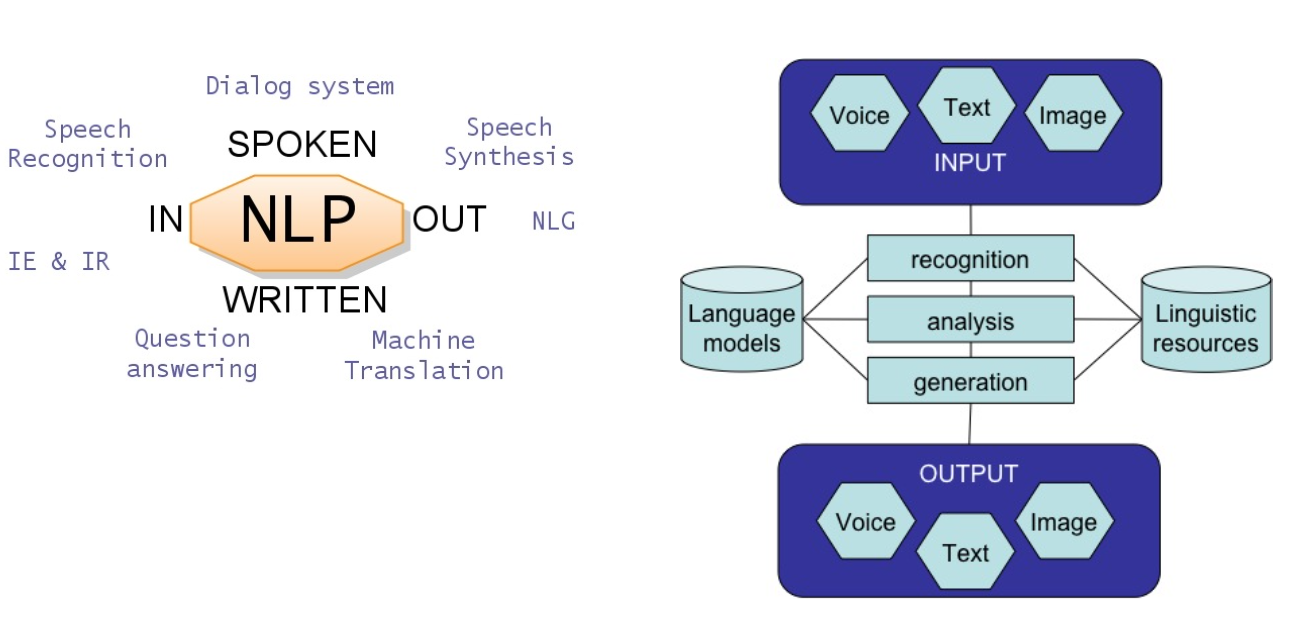
\includegraphics[width=\textwidth]{img/typical_tasks}
	\caption{Summary of typical NLP tasks}
	\label{fig:typical_tasks}
\end{figure}

There are two complementary approaches to NLP:
\begin{itemize}
	\item \textbf{Symbolic/linguistic/rule-based} approach.
	This approach is based on intensive use of language resources, with computer programs relying on rules hand-developed by linguists or other information specialists.
	\item \textbf{Statistical/ML} approach.
	This approach is based on empirical and automated techniques to learn models from data sources.
\end{itemize}
Historically, the rule-based approach came first, whereas the statistical approach appeared later with the rise of computing power.
It is often argued that \emph{hybrid} methods are most promising.
With the current advances in computing power and ML/DL, as well as the abundance (petabytes) of data, this could change.